\documentclass[midd]{thesis}

\usepackage{graphicx}
\usepackage{times}
\usepackage{url}
\usepackage{listings}

\lstset{basicstyle=\ttfamily\footnotesize,breaklines=true}

\graphicspath{ {images/} }

\bibliographystyle{plain}

\title {MiddGuard}

\author {Dana Silver}
\adviser {Professor Christopher Andrews}

\begin{document}

\maketitle

\begin{abstract}
Your abstract goes here.
\end{abstract}

\begin{acknowledgements}
Your acknowledgements go here.
\end{acknowledgements}

\contentspage
\tablelistpage
\figurelistpage

\normalspacing \setcounter{page}{1} \pagenumbering{arabic}

\chapter{Introduction}

Be able to create bespoke visualizations quickly.

\section{Visual Analytics}
\begin{enumerate}
  \item Why this is a useful tool in the context of visual analytics.
\end{enumerate}

\section{Previous Work on MiddGuard}
\subsection{VAST 2014}

Initial work on the MiddGuard framework began during summer 2014 as a research
project conducted by Christopher Andrews and Dana Silver. For a VAST 2014 Mini-Challenge
2 \cite{vast2014mc2} submission, we created a web interface to
visualize and analyze data from the challenge scenario. Data were preprocessed
using several disjoint Python scripts and the resulting manipulations were
persisted to a SQLite database. On the back-end of the web service, a simple
RESTful Python web server implemented with Flask \cite{flask} and Flask RESTful
\cite{flask-restful} queried the database and transformed data for various
front-end visualizations. The server also performed manipulations in addition
those in the preprocessing stage on a request-by-request basis based on analyst
input in the interactive visualizations.

An example of the flow between preprocessing scripts, back-end server, and
front-end visualization is how we identified points of interest in the
Mini-Challenge 2 geographical data. The VAST 2014 Challenge \cite{vast2014}
posited the following fictitous scenario:

\begin{quote}

In January, 2014, the leaders of GAStech are celebrating their new-found fortune
as a result of the initial public offering of their very successful company. In
the midst of this celebration, several employees of GAStech go missing. An
organization known as the Protectors of Kronos (POK) is suspected in the
disappearance, but things may not be what they seem.

\end{quote}

Available data for Mini-Challenge 2 included vehicle tracking data from
company cars, an ESRI shapefile of the island where GAStech is located, and an
illustrated tourist map of the island. Tracking data contained lists of
latitude, longitude, timestamp, and car ID. A preprocessing script iterated
through each trace's points, identified periods where a car was stopped for
greater than 120 seconds, and saved that coordinate as a destination for the
associated car. A visualization used TopoJSON \cite{topojson-spec} generated
from the shapefile and the tracking data to draw a map of the city overlayed
with cars' movements and destinations. By selecting a destination in the
visualization, an investigator could create a point of interest based on the
names of locations in the tourist map and persist the association of point of
interest and destination to the database. During the persistence step other
destinations within a certain radius would also be associate with that point of
interest.

The VAST 2014 submission was unsuccessful. Working on the tool described above
took most of the available time and investigators were not left with sufficient
time to complete the investigation and write up the results.

The first version of MiddGuard, which was developed in response to summer
research at Middlebury, attempted to generalize parts of the web server and
front-end that could be reused throughout multiple investigations, while keeping
the framework unopinionated with respect to the data it could handle. The
framework's primary features were automatic persistence to a database, data
transport between the server and connected web clients in real-time, centralized
data storage in the web browser, and visualization module loading/unloading in
the browser.

This version of MiddGuard achieved flexibility by automatically loading three
types of customizable packages. These were referred to as analytics, modules,
and models. Analytics were scripts that could be triggered by a remote procedure
call from a front-end visualization. They could be passed data from the
front-end. Using the VAST 2014 example, they were meant to handle computations
like finding other destinations near a point of interest.

Modules were front-end visualizations. JavaScript and CSS files required for the
visualization were declared in a package's \texttt{manifest.json} file. The
database was accessible on the front-end, with each table represented by a
Backbone.js collection. Modules could access collections using the global
\texttt{middguard.entities} object. Collections were updated in real-time over
WebSockets, so by listening to changes in a collection or the models it
contained, a visualization could update in real-time based on changing data on
the server. By extending a base MiddGuard View \cite{backbone} and registering
with MiddGuard by calling a function \texttt{middguard.module(name,
constructor)}, visualizations could be loaded and unloaded from the window with
a button click from MiddGuard's sidebar.

Models were the final piece of customization, intended to give the database
flexible schema to work with any data. Models were a combination of database
migrations and a Bookshelf.js \cite{bookshelf} model declaration. MiddGuard
included a \texttt{migrate} command to migrate models on a table-by-table basis,
applying the results a single database. The model declarations were patched to
emit WebSocket events on create, read, update, and delete events so that
analytics packages could be written to use the models, persist changes, and
communicate those changes to connected clients without needing to explicitly
alert connected clients. Relationships could be established between models using
a special \texttt{relationship} table that stored pairs of table names and row
ids.

\subsection{View Reference Counting}

\begin{enumerate}
  \item MiddGuard Version 1 (Summer 2014)
  \begin{enumerate}
    \item Reusable components
    \item Award/VAST 2015 challenge
  \end{enumerate}
\end{enumerate}


\chapter{Background}

\section{State of the Art}
  \begin{enumerate}
    \item Tools that currently exist and inspired MiddGuard.
    \begin{enumerate}
      \item Improvise
      \item Eagle Eyes
    \end{enumerate}
  \end{enumerate}

\chapter{The Framework}

\section{Overview}

MiddGuard is a web framework that enables software developers and analysts to
create the tools to conduct complex, data-driven investigations. It provides a
browser based front-end and web server back-end on top of which developers can
build customizable tools specific to their data and investigation. Data is not
uniform and investigating that data requires bespoke tools. MiddGuard,
rather than implementing all the specific tools necessary to address all
possible scenarios, provides the scaffolding on which developers can bring and
build their own tools. The user interface and web server that MiddGuard
implement create a simple environment to connect and use those tools
transparently and efficiently.

MiddGuard breaks the operations of a visual analytics based investigation into
two general steps: data transformation and data visualization. Data
transformation involves any function on the data that results in a different,
possible destructive, representation of the same dataset. These functions might
involve reading, filtering, aggregating, annotating, or reformatting the
dataset. As a general rule in MiddGuard, if the operation does not produce a
visualization, it is a transformation. Data visualization takes place after the
transformation steps, creating a visual, often interactive, representation of
the dataset. By implementing these two steps, developers can extend MiddGuard to
fit their data and investigation.

These extensions to MiddGuard are called modules. Modules are short pieces of
code that often live in a single file. We divide modules into two types to
represent data transformation and visualization respectively. The former is
called an analytic module, while the latter is a visualization module. Modules
implement a simple protocol that MiddGuard hooks into to use the code within the
framework. Analytic modules consist of code that runs solely on the web server.
Visualization modules contain code that runs in the web browser to render DOM
elements that make up its visualization.

Once the MiddGuard web server is running, investigators use these modules to
build a data-flow graph. Modules are the graph's nodes. Edges between nodes
describe data-flow from module to module. MiddGuard's web front-end comes with a
graph editor that investigators use to add modules to the graph and connect
modules to each other. Once added to the graph, a module has been instantiated
in the context of the graph and is called a node. Analytic nodes can be chained
from one to the next, making the graph a canvas to compose complex data
transformations from multiple analytic modules, each with a singular task.
Visualization modules can be connected to analytic nodes, which feed in data to
create the visualization.

Although modules are customizable and can be written for a particular
investigation, they are also reusable within the same graph, different graphs of
the same investigation, or multiple different investigations. Modules'
relationships to each other are managed by MiddGuard and defined by connections
in the graph, rather than hardcoded into the modules themselves. For example, a
developer could create a visualization module that renders a heatmap of two
entities' activity moving around a city. The module would be written to accept
input from Entity A, Entity B, and the data to draw the underlying city map. An
investigator can connect the heatmap to any two cars, people, bikes, etc. from
another dataset and render a heatmap with no additional development effort. As
developers and investigators use MiddGuard, they build up a library of these
reusable tools. In a an investigation where time is a factor, being able to
quickly plug in and test data transformations and visualizations promotes the
investigator's efficiency.

\section{Example: Using Tweets to Investigate Relationships}

An example of the data-flow model is using tweets to determine the relationships
between multiple people: Alice, Bob, and Carlos. We start by writing three
similar modules that use a JavaScript library to access the Twitter API and
download all of the tweets for each person, respectively. Between the three
modules we only need to change the Twitter handle for which we are downloading
tweets. We add a graph called ``Tweet Relationships'' then create nodes from
these modules and add them to the graph. We can use the number of times one user
mentions (such as @Bob) another as a metric for the relationship, so we write
another module called ``Mention Count'' that extracts mentions from each tweet
and creates a mapping from the Twitter user mentioned to the number of times
mentioned throughout the dataset. We add this module to the graph three times,
and connect one ``Mention Count'' node to each of Alice, Bob, and Carlos's tweet
download nodes. Already we are able to reuse ``Mention Count'' for each person's
tweets. Finally, we visualize the relationships. We can use a force directed
graph with a node for each person and strength of the edges proportional to the
number of times one mentioned the other. Our visualization module, ``Force
Directed Graph'' will take three inputs, one for each person. We create a node
in the graph from the ``Force Directed Graph'' module and connect each of the
outputs from our ``Mention Count'' nodes to the three inputs of ``Force Directed
Graph''. Like the ``Mention Count'' module, ``Force Directed Graph'' is reusable
and can be plugged into any three inputs.

At this point our graph is ready to produce data and a visualization. We work
from the data entry points to the visualization, running the tweet download
nodes, then the ``Mention Count'' nodes, then the ``Force Directed Graph''
visualization. The analytic nodes report when they are done so we know it is
safe to run their dependents. Running the node ``Force Directed Graph'' renders
the visualization next to our graph in the browser window.

\section{Collaboration}

MiddGuard not only enables single investigators to create and work with these
tools, but also has built in support for asynchronous and synchronous
collaboration between teams of investigators. The framework includes user
registration and authentication so multiple investigators can create accounts,
log in, and work on the same investigations with the same graphs and access to
the same data. All configuration and transformed data is persisted to a
database, so investigators can log in and work with each other asynchronously,
one picking up where the other left off. Investigators can also work together in
real-time. As edits to the data-flow model are persisted to the database, they
are pushed to all connected web clients and the user interface updates without a
refresh to reflect those changes.

Since developers can collaborate to build the investigation, it follows that
they should be able to collaborate to record conclusions from their analysis.
MiddGuard comes with an observations tool for investigators to record and share
observations about the analysis, creating a chronological record of what
investigators saw in the data and when they saw it. An investigator of the
tweet-based relationships from the previous example might record ``Alice appears
to have a close relationship with Bob. See the Force Directed Graph
visualization in the Tweet Relationships graph.'' Like graphs and data, these
observations are persisted to the database and pushed to all connected clients
in real-time.

\chapter{Implementation}

\section{Data-flow Programming}

MiddGuard's data-flow model allows arbitrary nodes, each with their own idea of
input and output, to be chained together in a graph of data transformations and
visualizations. Nodes are reusable units of code, so multiple instances of the
same type of node, or module, can coexist in a single investigation. Connections
between nodes allow data to pass between them.

\subsection{Nodes}

Nodes are at the heart of the data-flow model's implementation. In this section
we will address the implementation of analytic nodes. Visualization nodes and
their differences with respect to analytic nodes will be addressed in a
subsequent section.

Each node is representative of a function, called the handler, and the node's
dynamically generated context. The handler is a function exposed by the node's
backing module that performs a data transformation. Each nodes' respective
context has an input and an output component. In terms of inputs, the context is
a mapping from the names a node gives its own inputs to names of the outputs of
its incoming connections. For a node's output, the context is a mapping from a
generically named variable, \texttt{output}, to a specifically named table in
the database.

A node's inputs work at two levels, input groups and column-level connections. A
set of column-level connections is encompassed by an input group. Input groups
work at the table level, making a configuration based connection between two
tables in the database. The column-level connections map columns in an output
table to columns in an input table.

Each node has a corresponding table in the database. A mapping from an input
group to an output node creates a mapping from the name the input node (the
owner of the input group) has given that group to the table represented by the
output node. Within each input group are several column mappings, also mapped
from the names of input columns given by the input node to the names of columns
in the output node's table.

\subsection{Connections}

Connections a two-level protocol of node to node connections and
intra-connection name mappings.

The connections generated within the graph editor are stored in MiddGuard's
table of nodes, as a JSON string in the same row as their corresponding input
node. Listing \ref{lst:connectionjson} shows an example connection configuration
for one of the ``Time by Day/Hour'' nodes in the figure \ref{fig:grapheditor}.
The connections for ``Time by Day/Hour'' only have one input group, called
``tweets'', which is connected to the output node with id \texttt{9}. Node
\texttt{9} is the ``@DanaRSilver'' node. The \texttt{output\_node} field serves
as a foreign key referencing another row in the same table. Also stored within
the input group are the column-level connections between the input group and
output node \texttt{9}. These are stored in an array of objects called
\texttt{connections}. Each object within the \texttt{connections} array has an a
key \texttt{input} and a key \texttt{output}. The value of \texttt{input} is the
name the input node has given to the column and the value of \texttt{output} is
the name the output node has given to the column.

\begin{lstlisting}[caption={A node's connection configuration. The node has a connection from its input group ``tweets'' to the node with id 9.}, captionpos=b, label={lst:connectionjson}]
{
  "tweets": {
    "output_node": 9,
    "connections": [
      {
        "output": "handle",
        "input": "handle"
      },
      {
        "output": "tweet",
        "input": "tweet"
      },
      {
        "output": "timestamp",
        "input": "timestamp"
      }
    ]
  }
}
\end{lstlisting}

We considered multiple factors when deciding how to store nodes and their
connections in the database before deciding on a JSON string stored with the
connections' input node. We wanted a storage method that was portable,
efficient, and convenient. Portability meant that we could easily export the
configuration of nodes and connections to a text file so they could be read back
in and the graph could be reassembled in a different system. Efficiency was
determined by the number of database operations required to access the
configuration. This was important since we have to read and write connections
whenever a node is accessed or modified in the graph editor. Convenience meant
that it was not overly complex to access and modify the connections from a
programming perspective.

In addition to the JSON string storage method we implemented, we considered
storing connections and nodes in separate tables, with either each column-level
connection in its own row or each group of column-level connections in a row.
The former performed no grouping amongst column mappings, while the latter
grouped each input group's columns in a single row.

The first option (each column mapping has its own row) was appealing since it
took advantange of the relational database, using foreign keys to associate
column mappings with their nodes. However, this method is less portable since it
requires multiple steps to export all the node information and their associate
column mappings from the database to a structured text file. It is also less
efficient since it requires reading a row from the database for every column
mapping, in addition to a row for every node. Finally, it would be less
convenient to develop with because it would require more queries to the database
to obtain all the information to construct the graph than if we stored the
connection information close to the nodes.

For similar reasons, we ruled out the second option of storing all column level
connections in a row, grouped by their input group. This seemed like a poor
compromise between storing all column mappings separately and storing all
connection information with their nodes. We would lose the elegance of
conforming to the facilities of a relational database, and still have to query
the database multiple times to assemble a graph or export/import the data.

The implemented method of storing a node's connection in the same database table
row as the node, in a JSON string, satisfied all our requirements. It is
portable: JSON is common format to export human readable configuration. We can
simply query all nodes and write out their metadata and JSON string as
connections. It is efficient to access nodes and connections to construct a
graph. All of a graph's nodes and connections can be accessed by reading
\textit{n} rows from the database, where \textit{n} is the number of nodes in a
graph. It is convenient to work with this format, since all the connection data
for a node can be obtained by calling JavaScript's built-in \texttt{JSON.parse}
method on a node's connections column.

A node's connections can be edited in the graph editor until runtime, when a
node's handler funtion is executed. At this point, MiddGuard makes a query for
the node in the database and retrieves its stored connections. Parsing the
connections JSON string lets MiddGuard access the mapping of input groups to
output nodes and the mappings of column names between nodes. MiddGuard makes
additional queries to determine the table names of connected output nodes. With
just this information, MiddGuard can construct the dynamically generated context
to pass into the handler function. Listing \ref{lst:nodecontext} is a sample of
the context passed into one of the ``Time by Day/Hour'' nodes visible in figure
\ref{fig:grapheditor}. At the top level it includes \texttt{inputs} and
\texttt{table}. \texttt{inputs} is an object mapping each of the nodes input
groups to data about the connected output node. Within \texttt{inputs} are:
\texttt{knex}, an instance of the Knex.js SQL generator \cite{knexjs}, used to
access the table connected to an input group; \texttt{cols}, the column-level
mapping between the node's input group and the connected output node's column
names; and \texttt{tableName}, the name of the connected output node's table
name. \texttt{cols} and \texttt{tableName} are meant to give access to the
information available for more advanced queries, such as table joins.

The other top-level key in the context, \texttt{table}, gives access to the
output table for this node. Like each input group in \texttt{inputs}, it has a
\texttt{knex} accessor to generate SQL to query the database, and a
\texttt{name}, which is the node's own table name. \texttt{table} doesn't need a
column mapping, since the column names are the same as the ones the node has
assigned itself as outputs.

\begin{lstlisting}[caption={The context passed into a ``Time by Day/Hour'' node's handler function.}, captionpos=b, label={lst:nodecontext}]
{
  inputs: {
    tweets: {
      knex: [Object],            // database connection instance
      cols: {
        handle: 'handle',
        tweet: 'tweet',
        timestamp: 'timestamp'
      },
      tableName: 'download-tweets-danarsilver_1'
    },
    table: {
      knex: [Object],            // database connection instance
      name: 'aggregate-time_2'
    }
  }
}
\end{lstlisting}

Having to make additional queries to access output nodes' table names is a
potential source of ineffiency not addressed by our connections storage format.
A way around this would be to duplicate the table name each time it appears in a
connections JSON string. We decided against duplicating the data and in favor of
making additional database queries instead to avoid fragmenting the information,
should the table name change. Should we need to update a node's table name, it
can be done once for the row, rather than having to update the connections
string in all other connected nodes.

\begin{figure}[!ht]
  \centering
  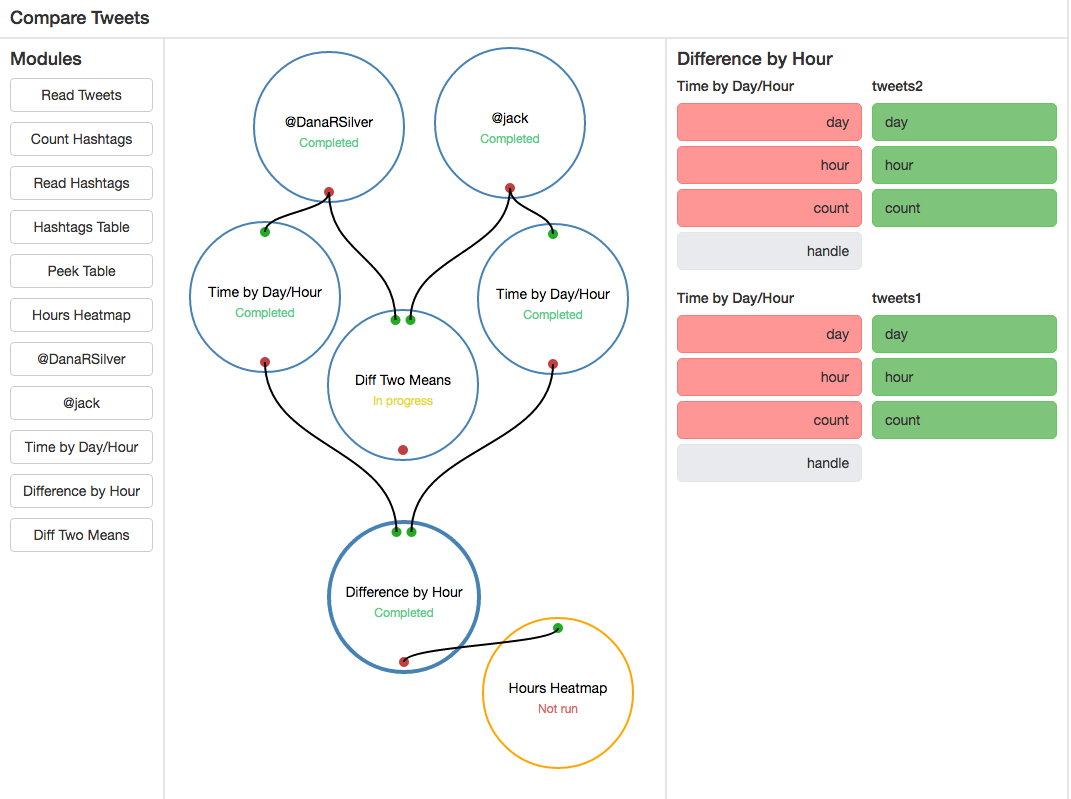
\includegraphics[width=1\textwidth]{compare-tweets-graph-editor-no-sidebar}
  \caption{MiddGuard's graph editor user interface, open on a graph named
  ``Compare Tweets''. On the left, the modules panel lists all loaded modules,
  from which nodes can be created. In the center, the graph editor canvas has
  seven nodes initialized from their respective modules, and connections between
  the nodes. On the right, the detail panel shows the column mappings between
  the ``Difference by Hour'' node and its connections to two
  ``Time by Day/Hour'' nodes.}
  \label{fig:grapheditor}
\end{figure}

\section{Visualization Nodes}

Visualization nodes, like analytic nodes, are added from modules in the graph
editor. Figure \ref{fig:grapheditor} has a visualization node with the label
``Hours Heatmap'' with an orange outline. Like analytic nodes, visualization
nodes have input groups that can be connected to output nodes, and column
mappings between the two nodes on the ends of the connections. The primary
difference between analytic nodes and visualization nodes is that the handler
for an analytic node is a single function that is called and run on MiddGuard's
back-end server, while the handler for a visualization node is a newly
instantiated Backbone.js View \cite{backbone} that is rendered in the web
client.

The instantiated view for a visualization node has an instance method called
\texttt{createContext}, which can be called to dynamically generate the context
for a view, just as the MiddGuard generates the context for an analytic node on
the back-end and passes it into the handler function. The context for a
visualization node has the same structure as that of an analytic node, less the
output \texttt{table}, since a visualization node's output is a visualization,
rather than a table of data.

Additionally, the \texttt{knex} key for each input group is replaced with an
instance of a Backbone Collection (with a key aptly named \texttt{connection}),
which can be used like the \texttt{knex} key to access the data from output node
connected to that particular input. MiddGuard instantiates a Backbone collection
for each analytic node and a corresponding endpoint on the back-end to transmit
the analytic node's data to the collection, as required by a visualization node.

A potential improvement in the implementation of visualization nodes would be to
only instantiate collections for analytic nodes that output to visualization
nodes. Other nodes' data will never be accessed, so it is not necessary to
maintain collections on the front-end or the endpoints on the back-end to
transmit data to them. However, this is a low-priority improvement since there
is little overhead in terms of memory usage to create an empty connection on the
front-end or add the event listeners that handle data transmission to Node.js's
event loop on the back-end.

\section{Visual Programming}

Figure \ref{fig:sidebar} shows the sidebar with the ``Graphs'' panel in
view and multiple graphs already created and listed below the new graph input.

\begin{figure}[!ht]
  \centering
  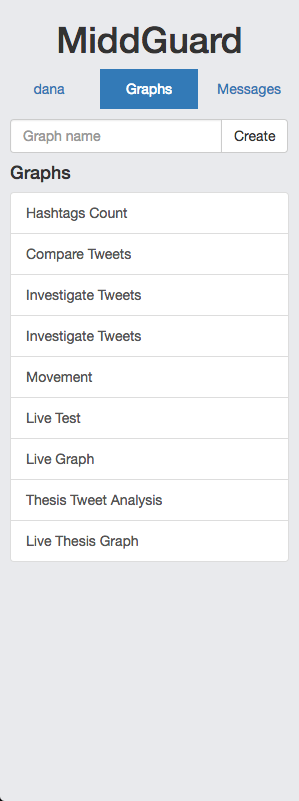
\includegraphics[width=0.5\textwidth]{sidebar-graphs-panel}
  \caption{MiddGuard's built-in sidebar with the ``Graphs'' panel in view.}
  \label{fig:sidebar}
\end{figure}

Visual programming abstracts away the details of the data-flow model within
MiddGuard as descibed in the previous sections, and the independent
implementation details of each node. A major motivation for MiddGuard is to
facilite quick construction of complex visual analytic tools. MiddGuard's system
for visual programming allows investigators to quickly compose data
transformations and visualizations. The visual component creates an expressive
representation of the steps to reproduce a visualization.

The visual programming interface takes place in the three panels of the graph
editor, seen in figure \ref{fig:grapheditor}. The left panel, titled
``Modules'', lists all modules from which nodes can be instantiated. Clicking a
module's button in the list adds a node of that type to the canvas in the middle
panel.

The middle panel's canvas is a free-form space limited by the height of the
window and a 500 pixel width constraint. Nodes, once added to the canvas, are
outlined circles that can be rearranged and connected to one another. Analytic
nodes and visualization nodes are outlined in blue and orange respectively, to
make them easy to differentiate.

Figure \ref{fig:annotatednode} shows an analytic node with all its elements for
user interaction in view. The cross in the upper left corner is used to drag the
node around the canvas. Allowing nodes to be draggable is a simple solution to
problem of node layout. A downside is the additional effort and time required on
the part of the user to position and reposition nodes in the canvas, but this is
outweighed by both its simplicity to implement over a layout algorithm and the
flexibility for the user to customize the graph view as best appeals to their
idea of the investigation.

The ``play'' button, located in the top right of each node abstracts both
analytic and visualization nodes' action. In an analytic node clicking play
calls its handler function. In a visualization node, the play button creates a
new instance of a visualization. Pressing a visualization node's play button
again removes that visualization from the browser window. Like the graph
editors, stack horizontally in the browser window. The user can scroll through
them from left to right.

While web scrolling is typically done vertically, we implemented view layout
horizontally, since MiddGuard was designed to be used on the same system used
for the preliminary VAST 2014 and VAST 2015 investigations. These investigations
used a system of three 27 inch displays arranged side by side
\cite{middguard-dinofunworld}.

Each node contains two text indicators: in the center of the node in black is
the node's module type. This is a visual indicator of the operation that will
occur or visualization that will be rendered. Just below is the node's status
indicator, one of ``Not run'', ``In progress'', or ``Completed'' in red, yellow,
or green, respectively. The status indicates whether the handler function has
already been invoked. Investigators ultimately use the node's status to
determine when a visualization is able to be rendered in the browser. Only once
all a visualizations dependent nodes have been run and have a status of
``Completed'', can a visualization be rendered.

The connections between nodes' inputs and outputs are key components in the
visual programming interface. They represent connecting code paths and passing
data from one node to another. A connection can be created from one node to
another by selecting one green input group indicator seen at the top of the node
in figure \ref{fig:annotatednode} and one red output indicator like the one seen
at the bottom of the same node. The selected input and output connectors are
outlined with a black stroke. It is possible to connect a node's input to its
own output, however this would result in no operation since the data required
for the input would not exist at runtime. Since nodes can accept input from
multiple outputs, hovering an input group indicator opens a tooltip with the
name of the input group under the mouse to aid the investigator in creating the
correct mapping.

Clicking a node widens its outline and opens the node's connections in the
detail panel, seen on the right of figure \ref{fig:grapheditor}. The detail
panel lists each input group's column-level connections, grouped by that input
group, and organized so output columns are on the left in red, and input columns
are on the right in green. When a connection is made in the graph editor,
MiddGuard attempts to automatically match columns based on the names. Any
columns that don't match appear below the matched ones in gray. Columns can be
connected manually in the same way as nodes: by clicking to select an output and
an input to connect. The columns names in each group re-render to indicate the
pairing after the connection has been made manually.

The similarity between interactions to edit connections at both the node and
column level and the color coding of inputs and outputs in both the graph editor
canvas and the detail panel is intentional, meant to make graph construction
intuitive for an investigator. The goal of visual programming is to reduce the
complications for an investigator to create a complex program. A familiar, easy
to learn user interface promotes quick, simple development and reduces the
cognitive load devoted to MiddGuard as a tool rather than the investigation
itself.

\begin{figure}[!ht]
  \centering
  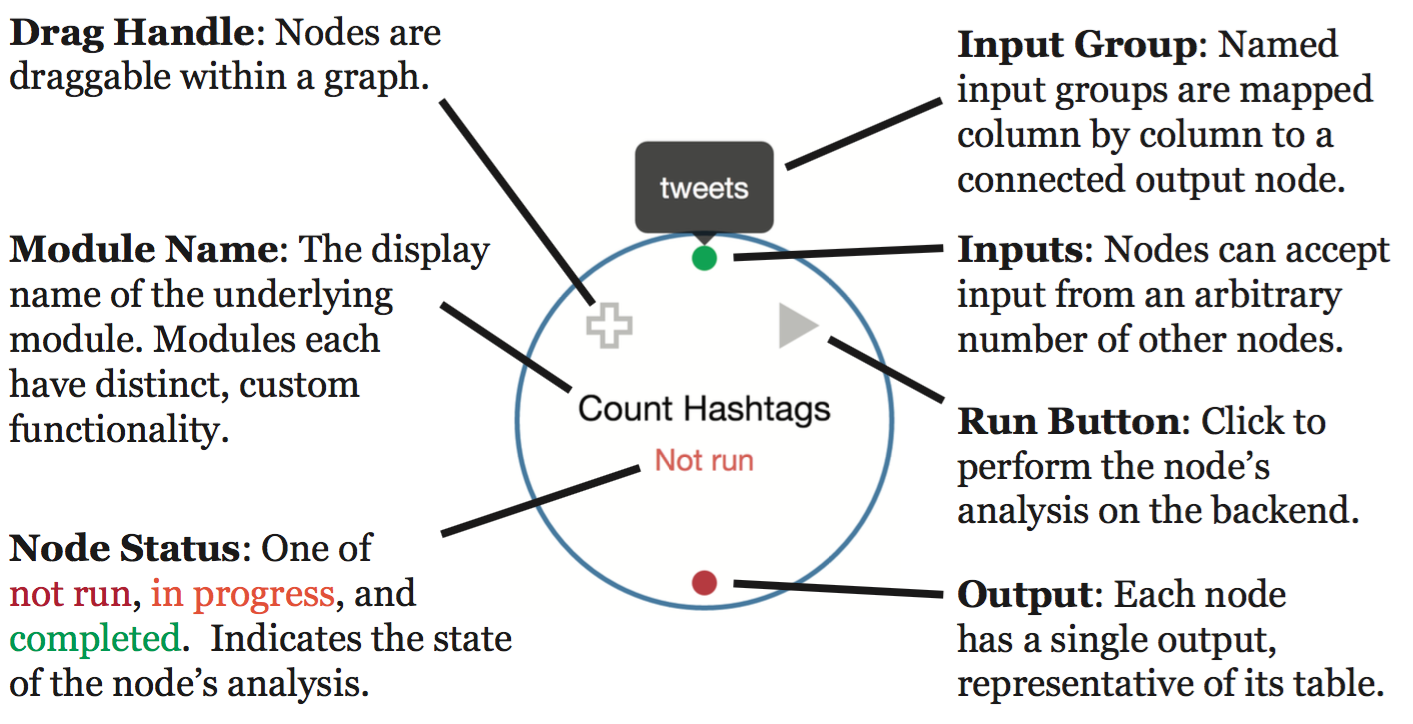
\includegraphics[width=1\textwidth]{middguard-analytic-node-annotated}
  \caption{An analytic node in a graph. Important features are annotated and the
  node's only input group, ``tweets'', is moused over to show its accompanying
  tooltip.}
  \label{fig:annotatednode}
\end{figure}

\section{Extensibility}

As mentioned before, the primary motivation for MiddGuard is to create a
framework that allows investigators and developers to quickly and effectively
create visual analytics tools. MiddGuard needs to be able to adapt to any
investigation with any types of data and visualizations. To support any data or
visualization, MiddGuard can register and load external code referred to as
modules. While visual programming is the user interface for analysts to quickly
put together an investigation with an expressive representation, the API for a
module is the user interface for developers who work with MiddGuard, and need to
quickly construct bespoke data transformations and visualizations.

Modules are the constructors from which nodes are initialized. They expose all
the metadata necessary to construct a node as well as the function or view that
will be called or rendered when the node's play button is pressed. Each node
contains a reference to the name of its constucting module so this metadata and
function can be accessed at runtime.

Modules themselves are short and designed to be written quickly. Figure
\ref{fig:analyticmodule} gives an example of an analytic module that bins tweets
by the day of the week and hour of their timestamp. This module performs the
final step of analysis in the ``Compare Tweets'' graph of figure
\ref{fig:grapheditor} before data is fed into the visualization.

An analytic module can be as simple as one JavaScript file that exports the few
objects as in figure \ref{fig:analyticmodule}. Those exports include an array
of inputs the module can accept, grouped by input group. Each input group
contains a list, \texttt{inputs}, of the attributes the module requires for each
member of the input group. The second export is an array of output attributes
for each member element the module will output.

The outputs correspond directly to the contents of the third export, a function called \texttt{createTable}. The \texttt{createTable} function is used to create the backing table for a node. All nodes

\begin{figure}[!ht]
  \centering
  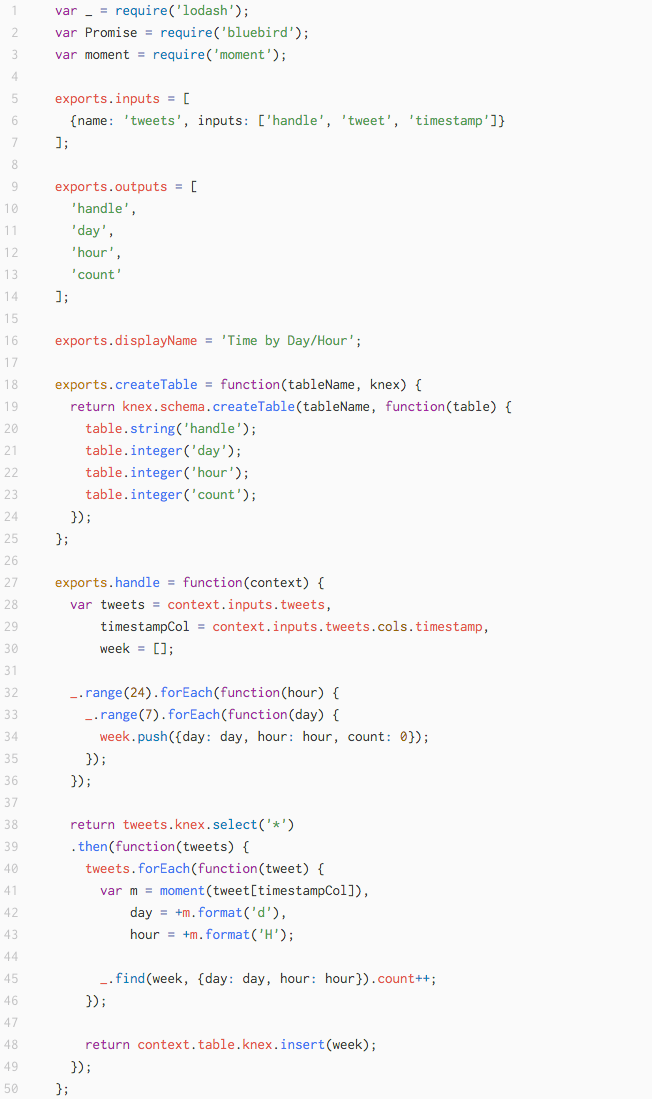
\includegraphics[width=.85\textwidth]{analyticmodule}
  \caption{Code for an example analytic module.}
  \label{fig:analyticmodule}
\end{figure}

\section{Real-time Collaboration}

MiddGuard supports asynchronous and synchronous collaboration between multiple
developers. Asynchronous collaboration is common in a web appliation. For
example, User A makes changes, which are persisted to a data store. User B logs
in some time later and the changes User A made are loaded from the database so
User B can view them.

Synchronous collaboration is more difficult. Web application communications are
largely based on the HTTP protocol. Data is transferred from the web server to
the client in an HTTP session, which is made up of a request from the client and
a response from the server. The client must initiate an HTTP request before the
server can send data. This is problematic for real-time communications. Like in
the asynchronous example, User A might make a change, which should be
immediately pushed to all other connected clients. User A can make an HTTP
request to tell the server about the change, but there is no way for the server
to tell other clients about the change immediately. With HTTP, User B must
explicitly request the update, which requires either knowing when to check for
an update (unreasonable) or continuously polling the server for changes
(inefficient).

WebSockets solve real-time communications, and are implemented in place of HTTP for all of MiddGuard's server-client communications, besides authentication.

  \begin{enumerate}
    \item Dataflow programming
    \item Visual programming
    \item Collaborative/real-time
    \item Extensibility
    \begin{enumerate}
      \item Front-end views
      \item Back-end analytic nodes
    \end{enumerate}
    \item Reusable nodes (agnostic of input/output data)
    \item Technology choices
  \end{enumerate}

\section{Technology}
  \begin{enumerate}
    \item Node.js
    \item Relational database (instead of NoSQL)
    \item Socket.io
    \item ORM
    \item Backbone.js
  \end{enumerate}

\chapter{Discussion}

\section{Use Case}

\begin{enumerate}
  \item Test/example case (tweet analysis)
  \item Ease of use for developer
  \item APIs exposed on front-end and back-end
\end{enumerate}

\section{Areas for Improvement}

\begin{enumerate}
  \item Use in real investigation (VAST Challenge 2016)
  \item Room for improvement
  \begin{enumerate}
    \item Better caching on front-end to help developers optimize DOM/memory
    usage
    \item Have to see if there is any else I don't have time to implement
  \end{enumerate}
\end{enumerate}

\chapter{Conclusion}
  \begin{enumerate}
    \item Revisit points from previous sections
    \item Why MiddGuard is an important visual analytics tool
    \item Open source prospects
  \end{enumerate}

\appendix
\chapter{Chapter 1 of appendix}
Appendix chapter 1 text goes here

\bibliography{thesis}

\end{document}
